\section{Machine-Learning}

\subsection{Classification or Regression}
In machine learning there are two type of functions approximators, classifications and regressions. Classification can output any value from a finite set and this method was previously used with $CS=\{0.001;0.01;0.1;0.5\}.$ Regression can output any number from a infinite set of candidates so it can be seen as classification algorithm where the number of candidates grows to infinity. But one has to wonder, Is it better to use less or more chunk sizes candidates. In [0] chunk sizes of $\{0.01;0.01;0.1;0.5\}$ have proven to be successful but can we improve performance by adding more candidates? If the variance of time is null than we have:

$$CS \subset CS' \Rightarrow \underset{cs \in CS'}{\min}t(X_i,cs)\leq \underset{cs \in CS}{\min}t(X_i,cs) \, \, \forall i$$

Which is to say that adding new candidates should always give a smaller or equal minimum of time. However, as seen earlier, there is variance in time measurement but we can hope that the variance is small enough to ensure that the statement is still true. This is my main hypothesis that will be tested:\\

HYPOTHESIS: Adding more candidates to $CS$ will reduce the execution times of hpx-loops.


 One way to test this assertion is to try a classification algorithm and adding more than 4 candidates but this becomes unpractical as generating data for many candidates takes longer. As an example data with 8 candidates takes around twice as long to generate as data with 4 candidates. Also, classification algorithms tends to reduce in accuracy the more candidates you add. However, if a regression algorithm is used, we technically have a set $CS$ which is infinite, even if we only use  4 or 5 candidates in the training set. This is because regression can interpolate between two candidates. For example if the candidates used when training are $\{0.01;0.1;0.5\}$ a regression could output any value in between like 0.0245879097 or 0.3333453 instead of being restricted to the finite set $\{0.01;0.1;0.5\}$.
 So let me rephrase the hypothesis:
 
 HYPOTHESIS(rephrase): Using a regression algorithms will give smaller execution times than classification algorithms.
 
  The goal of this analysis will be to confirm or infirm this hypothesis.


\subsection{Matrix Multiplication data-set}

The 4 regression algorithms that were studied on the matrix multiplication data-set are Support Vector Regression, Neural Network Regression, k-Nearest-Neighbors Regression and Random Forest Regression. To compare the performance of these algorithms, the k-fold cross validation has been used. In this method, you divide your data-set into k subsets and than you train the regression on (k-1) subsets and use the last subset as a testing set on which the regression will be evaluated. The measure of the error will be done by scikit's $MeanSquaredError()$ which outputs the mean of the squared error between the test subset and the predictions.

$$MSE(\hat{f})=\frac{1}{N_\text{test}}\sum_{i=1}^{N_\text{test}}(y_i-\hat{f}(X_i))^2$$

Where $\hat{f}$ represent the regression function which is an approximation of $f$, $X_i$ represent the features for an experiment $i$, $cs_i$ represents the target values and $N_{test}$ represents the number of experiments in the test set. It is important to note that to train regression algorithms, you need target values which are on the same scale. To solve this issue a logarithmic scaling is used on the targets values. This means that the error expressed will be the error of the logarithm. This is very hard to visualize but the goal is to compare models so we simply need to compare the errors. The chunk-size is obtained by applying the exponential function to the result of the regression.
Here are some results when using the data used to generate  figure [5]. A set of 64 experiments of matrix multiplication with sizes of 100,200,300,400, 500,600,700,800 and 2,4,6,8,10,12,14 threads.$CS=\{0.5;0.125;0.03125;0.0078125;0.001953125\}$

\begin{table}[h]
	\centering
	\caption{MSE on 64 experiments of matrix multiplicaition applications with logarithmic scaling using k-fold cross validation}
	\label{my-label}
	\begin{tabular}{|c|c|c|c|c|}
		\hline
		& SVR           & Neural Network & K-Nearest-Neighbors & Random Forest \\ \hline
		k=10 & 1.78+-1.14  & 1.72+-0.91    & 1.28+-1.31        & 1.55+-1. \\ \hline
	\end{tabular}
\end{table}

By using this metric, we can see that the k-Nearest-Neighbors and the Random Forest are the two best algorithms. I believe this is cause by the fact that these functions are piece-wise constant instead of being continuous like SVR and Neural-Network regression. However, the MSE is not a good metric to understand what happens locally when fitting the data. To better understand what happens locally, a graph of Ydata vs Yprediction can be used. In such graphs, cross validation is once again used but now the prediction are outputted. Each color represent a different test set.

\begin{figure}[H]
	\centering
	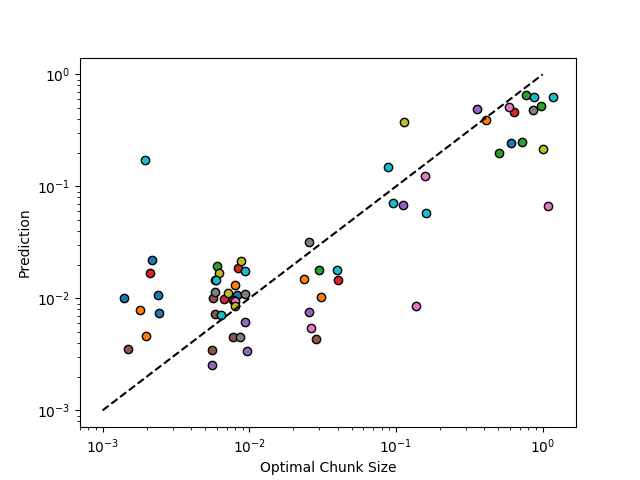
\includegraphics[width=120mm]{images/KNNR_eval.png}
	\caption{k-Nearest-Neighbors predictions vs reality using cross validation with 10 subsets }
\end{figure}

\begin{figure}[H]
	\centering
	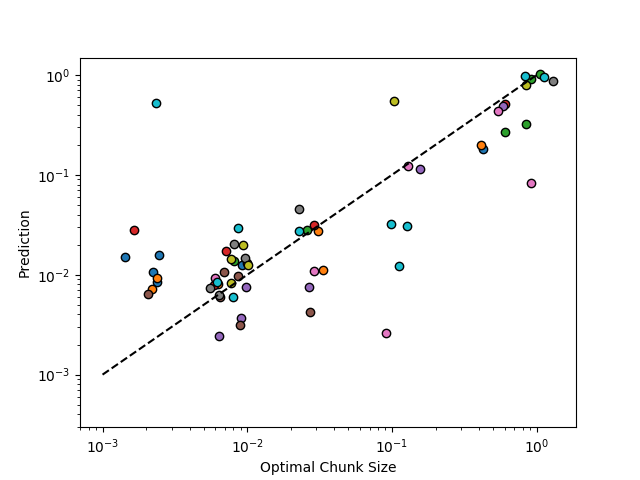
\includegraphics[width=120mm]{images/RFR_eval.png}
	\caption{Random forest predictions vs reality using cross validation with 10 subsets }
\end{figure}

We can see with these graphs that both algorithms are having similar results. However, calculating the error on chunk size is one thing but how does this error translate to execution time? The following measure I will call $Loop\_Total\_Time()$ will be used:

$$Loop\_Total\_time(\hat{f})=\sum_{i=0}^{N_{exp}} t(X_i,\hat{f}(X_i))$$

where $i$ represent a given experiment, $\hat{f}(x_i)$ is the predicted chunk size. $t$ is the execution time of a hpx $for\_each()$ loop with features $X_i$ and using the prediction of the machine learning as chunk size. To make this measure, the predictions on the experiments are obtained in python using k-fold cross validation, then the predictions are used as chunk-sizes on hpx $for\_each$ loops. However, this is an approximation because it doesn't include the time used to make the predictions and because the regressions are not fully implemented in hpx. Even though it's not fully representative of the performance of these algorithms if they were implemented in hpx, this measure is still a useful tool to see if interpolating between chunk-size candidates really improves performances. To verify the hypothesis, 2 regression algorithms were compared to the multinomial classification algorithm which is already fully implemented in hpx. All 3 algorithms are compared to the minimal time which is the summation of all the minimum times for each experiment in the data set.

\begin{table}[h]
	\centering
	\caption{Total execution times (s) on hpx for-loops using the predictions of 3 machine learning algorithms using k-fold cross validation}
	\label{my-label}
	\begin{tabular}{|c|c|c|c|c|}
		\hline
		& Minimal time &K-Nearest-Neighbors & Random Forest &Multinomial Classification\\ \hline
		k=10 & 9.86
		&10.07+-.16  & 9.95 s+-0.09 & 11.99+-0.4\\ \hline
	\end{tabular}
\end{table}

Here we can see that both algorithm regression have similar execution times. In fact, the difference between their execution time is lower than the uncertainty of the measurements and therefore we cannot conclude that one is better. However we can see that they both perform better than the Multinomial Classification. 

\begin{figure*}[h]
	\centering
	\begin{subfigure}[b]{0.515\textwidth}
		\centering
		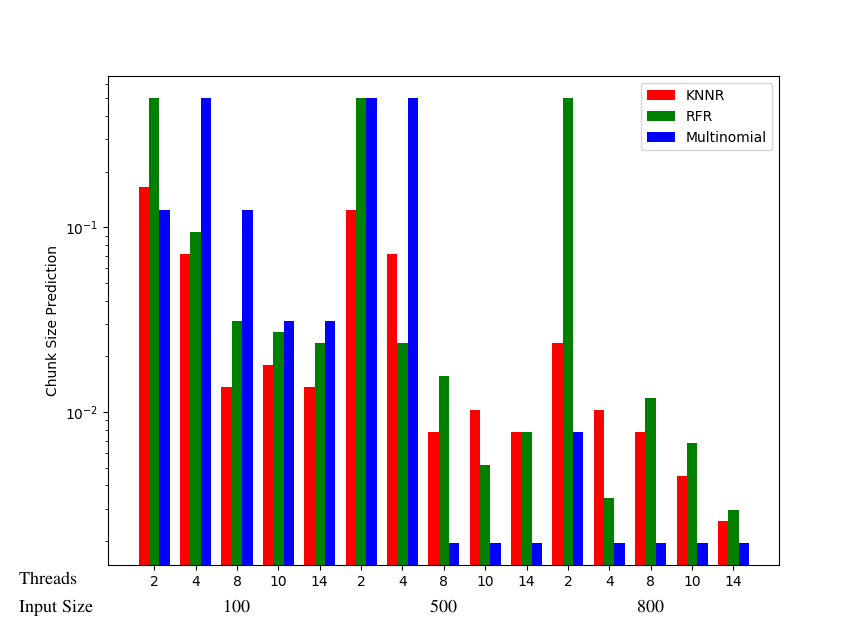
\includegraphics[width=\textwidth]{images/matrix_mult_prediction_bars.png}
		\caption[Network2]%
		{{Chunk sizes}}    
	\end{subfigure}
	\hfill
	\begin{subfigure}[b]{0.475\textwidth}  
		\centering 
		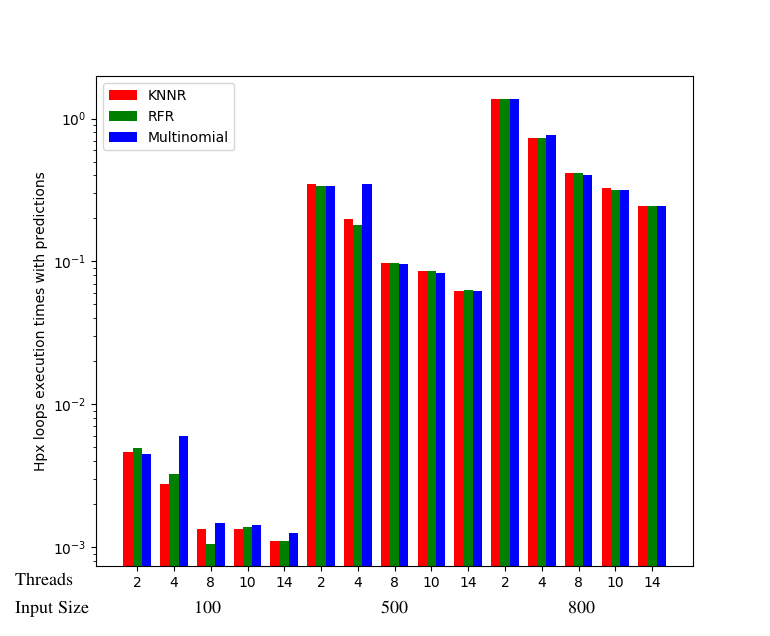
\includegraphics[width=\textwidth]{images/matrix_mult_times_bars.png}
		\caption[]%
		{{HPX loops execution times}}    
	\end{subfigure}
	\caption{Chunk sizes predicted by 3 machine-learning algorithms on Matrix Multiplication functions (a) and the resulting Execution times measured on hpx for-loops (b)} 
	
\end{figure*}



Resulting from this analysis, it seems that predicts 0.5 on more than 2 threads which never happens with the 2 regressions. This is because the two regressions algorithms take averages in the feature space so they are less likely to predict the highest chunk size 0.5. Predicting 0.5 is very risky because:

$$cs>\frac{1}{\text{number of threads}} \Rightarrow \text{miss-classification error}$$

 When you have $cs>\frac{1}{\text{number of threads}}$, it means that some CPU's are inactive since you don't divide your job into enough chunks to split to all available CPU's. Hence, predicting 0.5 is a high risk because if you are on more than 2 threads, it is a guaranteed error for big algorithms. Since there is less variance on 2 threads, it means that the reward for rightly predicting a  0.5 on 2 threads is smaller than the loss for wrongly predicting a 0.5 on more than 2 threads.
This miss-classification can be manually corrected after the multinomial classification prediction by reducing the chunk size until we have $cs\leq \frac{1}{\text{number of threads}}$. The chunk size obtained may not be the best one, but at least all the CPU's will be active. This will be refereed to as Multinomial Classification corrected.

\begin{table}[h]
	\centering
	\caption{Total execution times (s) on hpx for-loops using the predictions of 3 machine learning algorithms using k-fold cross validation}
	\label{my-label}
	\begin{tabular}{|c|c|c|c|c|}
		\hline
		& Minimal Time &K-Nearest-Neighbors & Random Forest &Multinomial Class Corrected\\ \hline
		k=10 &9.86 & 10.07+-0.16  & 9.95 s+-0.09 & 10.18+-0.09\\ \hline
	\end{tabular}
\end{table}

\begin{figure*}[h]
	\centering
	\begin{subfigure}[b]{0.5\textwidth}
		\centering
		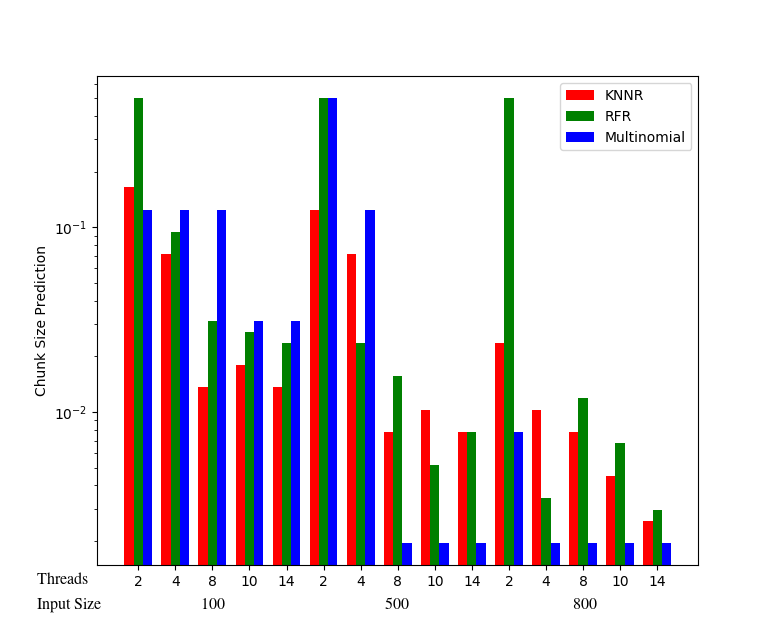
\includegraphics[width=\textwidth]{images/matrix_mult_corrected_predictions_bar.png}
		\caption[Network2]%
		{{Chunk sizes}}    
	\end{subfigure}
	\hfill
	\begin{subfigure}[b]{0.49\textwidth}  
		\centering 
		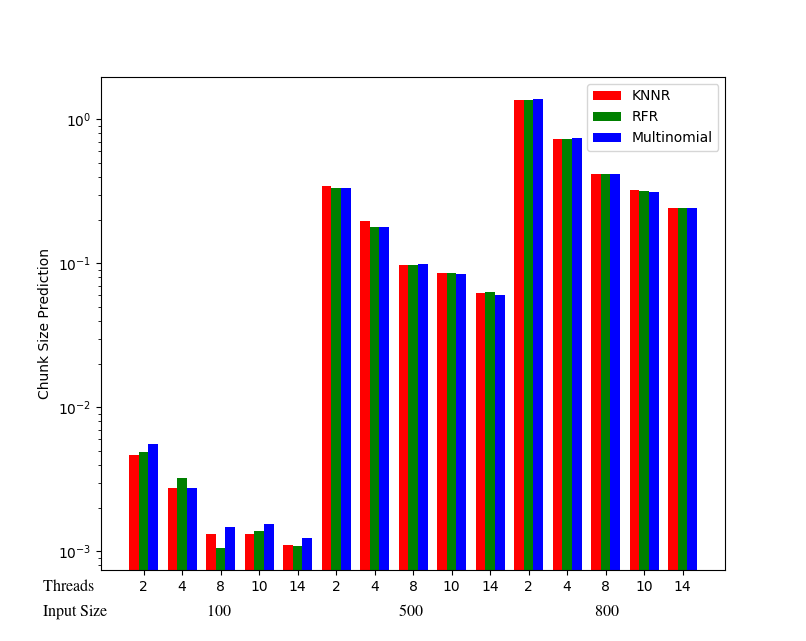
\includegraphics[width=\textwidth]{images/matrix_mult_corrected_times_bar.png}
		\caption[]%
		{{HPX loops execution times}}    
	\end{subfigure}
		\caption{Chunk sizes predicted by 3 machine-learning algorithms on Matrix Multiplication functions (a) and the resulting Execution times measured on hpx for-loops (b)} 
	
\end{figure*}

Here we can note that by manually reducing the aberrant chunk sizes has improved performances but we can still see that the classification has  a longer execution times in some instances. These instance happen to be the ones where the chunk size was manually reduced. However, it cannot be manually reduced any further because we don't know what is the best chunk size. The time difference for these errors is now smaller It is important to note that the color blue is not significant in this graph since its magnitude is around the variance of the data. This can be said because there are blue dots on the doted-line.
\subsection{1D stencil algorithm}
For this function, the multinomial corrected algorithm is compared to the two other regressions:

\begin{table}[h]
	\centering
	\caption{Total execution times (s) on hpx for-loops using the predictions of 3 machine learning algorithms with stencil function using k-fold cross validation}
	\label{my-label}
	\begin{tabular}{|c|c|c|c|c|}
		\hline
		& Minimal Time &K-Nearest-Neighbors & Random Forest &Multinomial Class Corrected\\ \hline
		k=10 & 93.57&94.65+-2.16  & 95.2 s+-1.98 & 99.32+-3.04\\ \hline
	\end{tabular}
\end{table}
\begin{figure*}[h]
	\centering
	\begin{subfigure}[b]{0.5\textwidth}
		\centering
		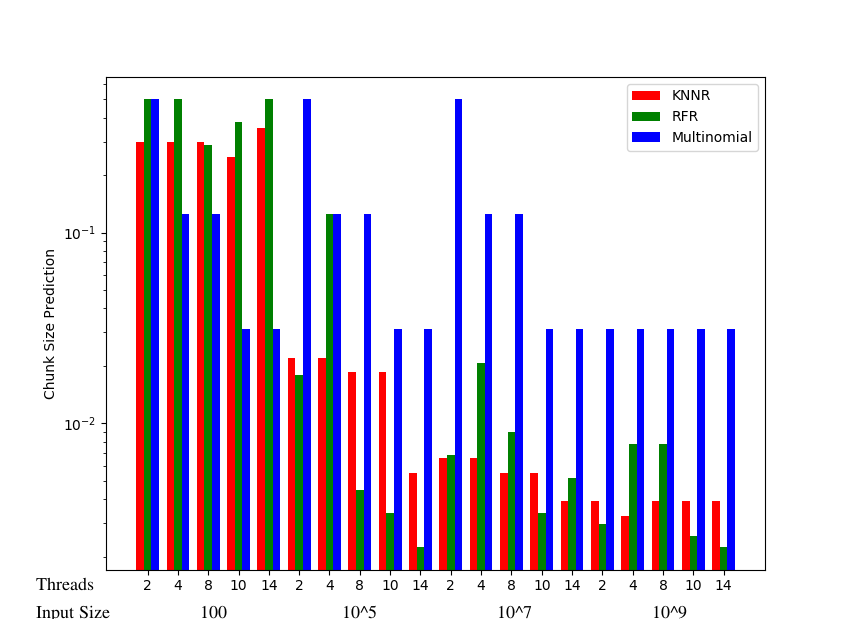
\includegraphics[width=\textwidth]{images/stencil_predictions_bars.png}
		\caption[Network2]%
		{{Chunk sizes}}    
	\end{subfigure}
	\hfill
	\begin{subfigure}[b]{0.49\textwidth}  
		\centering 
		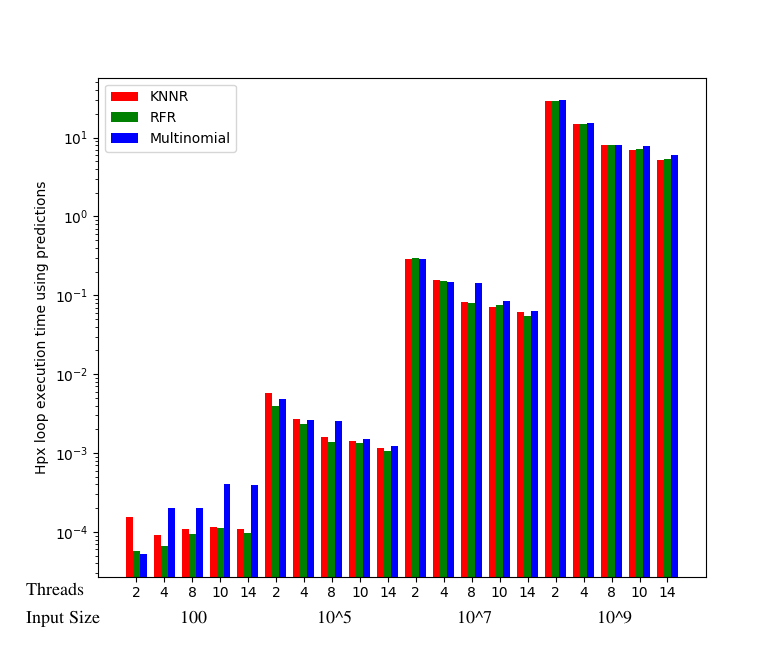
\includegraphics[width=\textwidth]{images/stencil_times_bars.png}
		\caption[]%
		{{HPX loops execution times}}    
	\end{subfigure}
	\caption{Chunk sizes predicted by 3 machine-learning algorithms on Stencil functions (a) and the resulting Execution times measured on hpx for-loops (b)} 
\end{figure*}
\subsection{Data Set with multiple functions}

On this data set, the Mean Square Error has once again been measured on the 2 selected regressions:

\begin{table}[h]
	\centering
	\caption{Mean Squared Error on 278 experiments with logarithmic scaling on $CS$ using k-fold cross validation}
	\label{my-label}
	\begin{tabular}{|c|c|c|}
		\hline
		& K-Nearest-Neighbors & Random Forest \\ \hline
		k=10  & 2.18+-1.1        & 1.5+- 0.45 \\ \hline
	\end{tabular}
\end{table}
\begin{figure}[H]
	\centering
	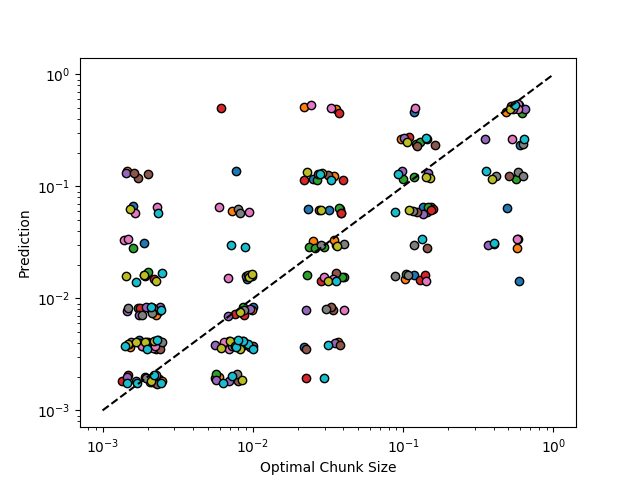
\includegraphics[width=120mm]{images/KNNR_eval_big.png}
	\caption{Evaluation of Nearest-Neighbors with 2 neighbors}
\end{figure}

\begin{figure}[H]
	\centering
	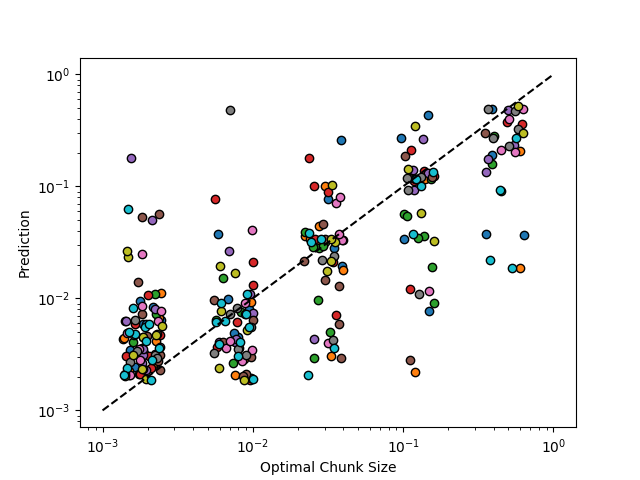
\includegraphics[width=120mm]{images/RFR_eval_big.png}
	\caption{Evaluation of random forest}
\end{figure}

The number of neighbors has been set to 2 because it was the value that minimized the MSE. However it is still quite big for k-Nearest-Neighbors relative to Random Forest. I believe it performs worse in that scenario because of the prepossessing on the big data set. In fact not normalizing the features gave a MSE of 1.67. It is normal that kNN is sensible to preprocessing and not RandomForest because it calculates Euclidean distance between points in the feature space. However I have decided to normalize the data nonetheless because the features are on different scales. The exact reason why kNN performs better without normalization could be studied on its own.
\\

Now let's see how this error in prediction relates to execution times. Once again the regressions are compared to Multinomial Classification:


\begin{table}[h]
	\centering
	\caption{Total execution times (s) on hpx for-loops with the predictions of 3 machine learning algorithms on 278 experiments using k-fold cross validation}
	\label{my-label}
	\begin{tabular}{|c|c|c|c|c|}
		\hline
		& Minimal Time&K-Nearest-Neighbors & Random Forest &Multinomial Class Corrected\\ \hline
		k=10  &312.01&
		 355+-4        & 344+- 4&356+-13 \\ \hline
	\end{tabular}
\end{table}

Like all previous results, multinomial classification is worst than the other algorithms. At it point in the project, it was discovered that there was no use of bias inside the multinomial model. The algorithms requires the computation of a linear function $W X$ where $W$ represents the weights which are parameters that need to be optimizes. Adding a bias consist of changing this function to an affine function $WX+b$ where $b$ is called the bias. Let's see how adding a bias improves the results:

\begin{table}[h]
	\centering
	\caption{Total execution times (s) on hpx for-loops with the predictions of 3 machine learning algorithms on 278 experiments using k-fold cross validation}
	\label{my-label}
	\begin{tabular}{|c|c|c|c|c|}
		\hline
		& Minimal Time&K-Nearest-Neighbors & Random Forest &Multinomial Class Corrected bias\\ \hline
		k=10  &312.01&
		355$\pm$4        & 344$\pm$ 4&341$\pm$4 \\ \hline
	\end{tabular}
\end{table}
We can see that simply adding a bias to the algorithm reduced the execution time on hpx loops by a huge factor. It has now become the best algorithm on the big data set. It may the best on all experiments, but it's still interesting to study the results on each type of function to see if it performs better on all lambda functions:
\newpage
\subsubsection{Nothing}

\begin{table}[h]
	\centering
	\caption{Total execution times (s) on hpx for-loops with the predictions of 3 machine learning algorithms on Nothing function using k-fold cross validation}
	\label{my-label}
	\begin{tabular}{|c|c|c|c|c|}
		\hline
		& Minimal Time&K-Nearest-Neighbors & Random Forest &Multinomial Class Corrected bias\\ \hline
		k=10  &0.6&
		0.604$\pm$0.021       & 0.6199$\pm$0.025&0.606$\pm$0.025 \\ \hline
	\end{tabular}
\end{table}

\begin{figure*}[h]
	\centering
	\begin{subfigure}[b]{0.5\textwidth}
		\centering
		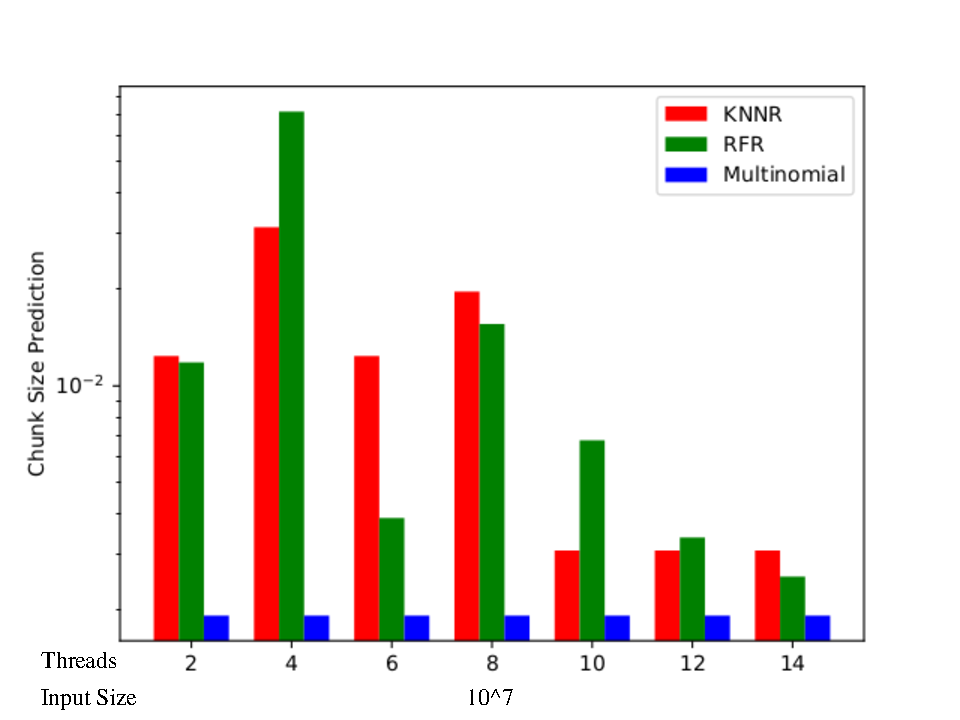
\includegraphics[width=\textwidth]{images/bars_nothing_cs.pdf}
		\caption[Network2]%
		{{Chunk sizes}}    
	\end{subfigure}
	\hfill
	\begin{subfigure}[b]{0.49\textwidth}  
		\centering 
		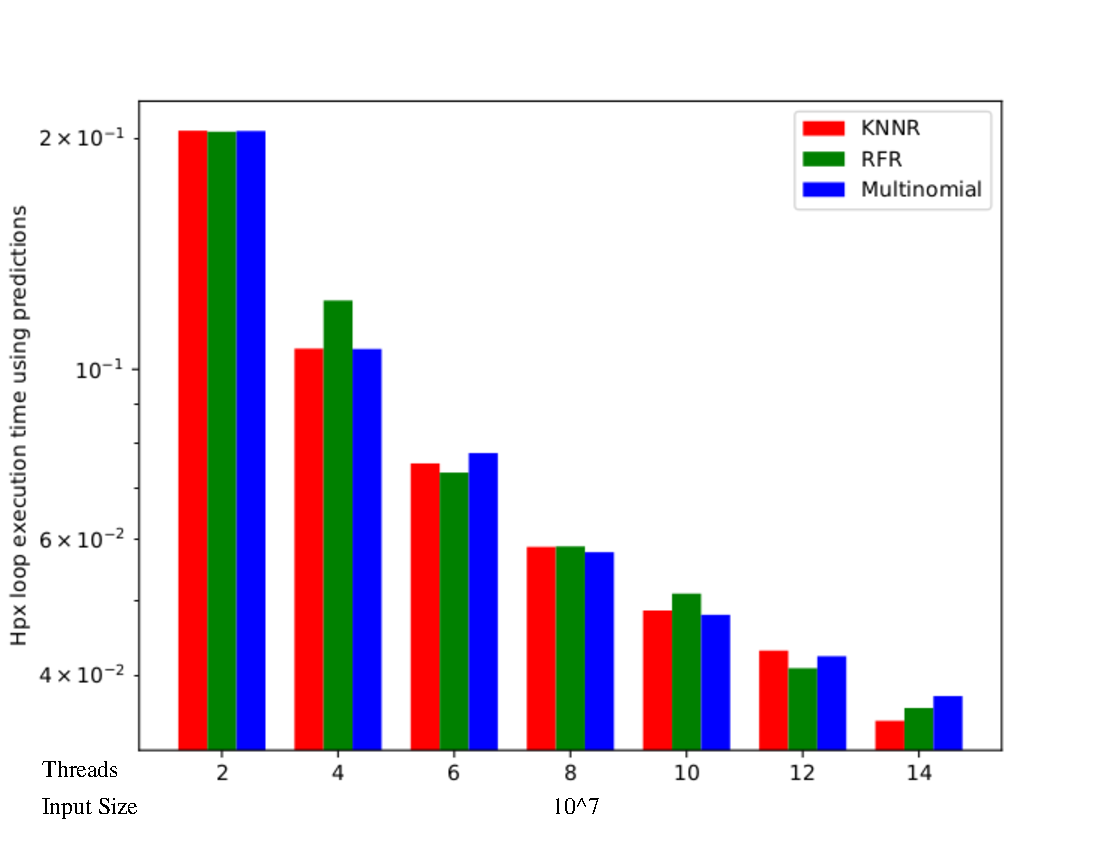
\includegraphics[width=\textwidth]{images/bars_nothing_times.pdf}
		\caption[]%
		{{HPX loops execution times}}    
	\end{subfigure}
	\caption{Chunk sizes predicted by 3 machine-learning algorithms on Nothing functions (a) and the resulting Execution times measured on hpx for-loops (b)} 	
\end{figure*}
The results for the 3 algorithms are very close but Random Forest predicted 0.5 on 4 threads which and add a bigger execution time as a result. It is interesting to see that Multinomial Classification always predicts the smallest chunk size. This is because the execution times between $\frac{1}{512}$ and $\frac{1}{128}$ are very close so the algorithm converged too early. This didn't seem to affect that much the total time measured on hpx for-loops.
\newpage
\subsubsection{Swap}

\begin{table}[H]
	\centering
	\caption{Total execution times (s) on hpx for-loops with the predictions of 3 machine learning algorithms on Swap function using k-fold cross validation}
	\label{my-label}
	\begin{tabular}{|c|c|c|c|c|}
		\hline
		& Minimal Time&K-Nearest-Neighbors & Random Forest &Multinomial Class Corrected bias\\ \hline
		k=10  &0.091&
		0.101$\pm$0.036       & 0.099$\pm$0.036&0.107$\pm$0.037 \\ \hline
	\end{tabular}
\end{table}

\begin{figure*}[h]
	\centering
	\begin{subfigure}[b]{0.5\textwidth}
		\centering
		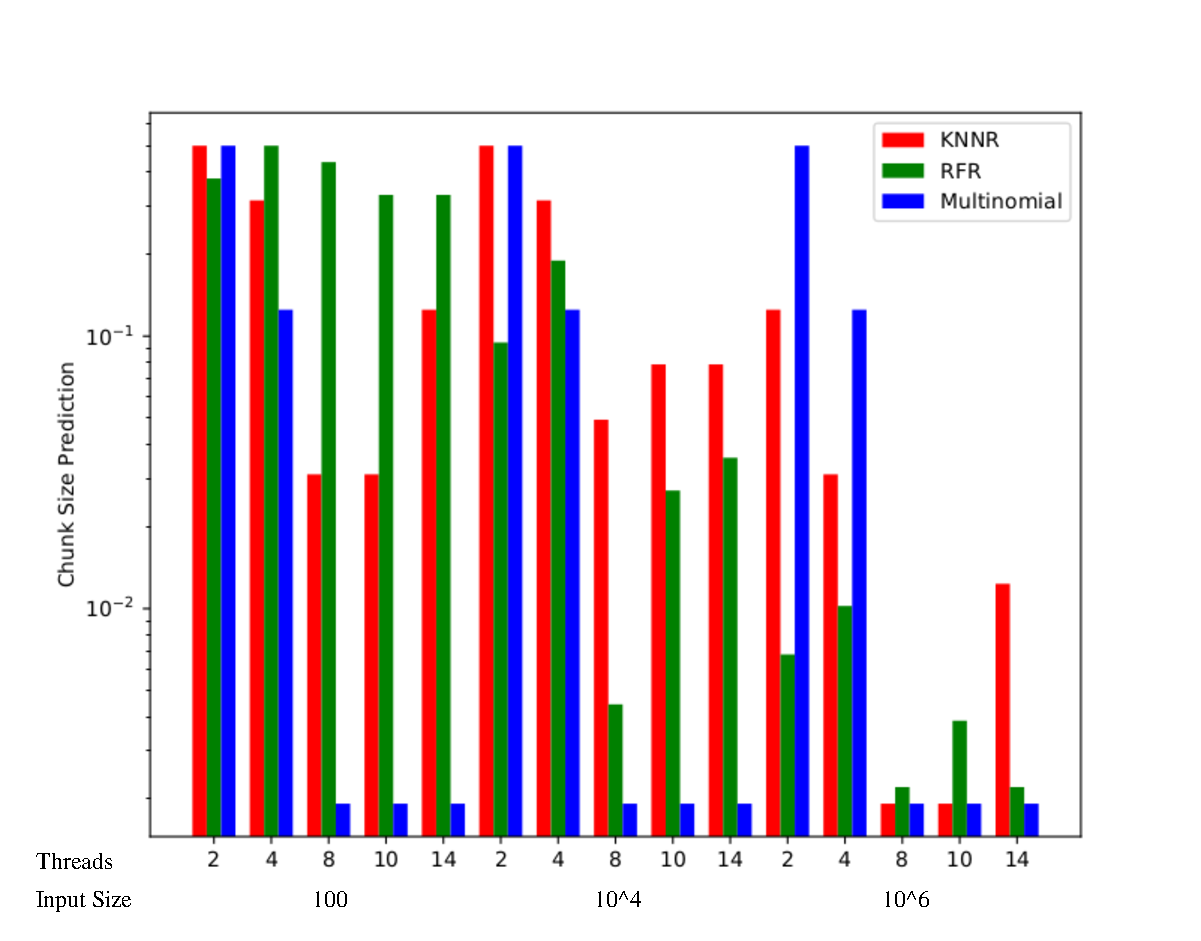
\includegraphics[width=\textwidth]{images/bars_Swap_cs.pdf}
		\caption[Network2]%
		{{Chunk sizes}}    
	\end{subfigure}
	\hfill
	\begin{subfigure}[b]{0.49\textwidth}  
		\centering 
		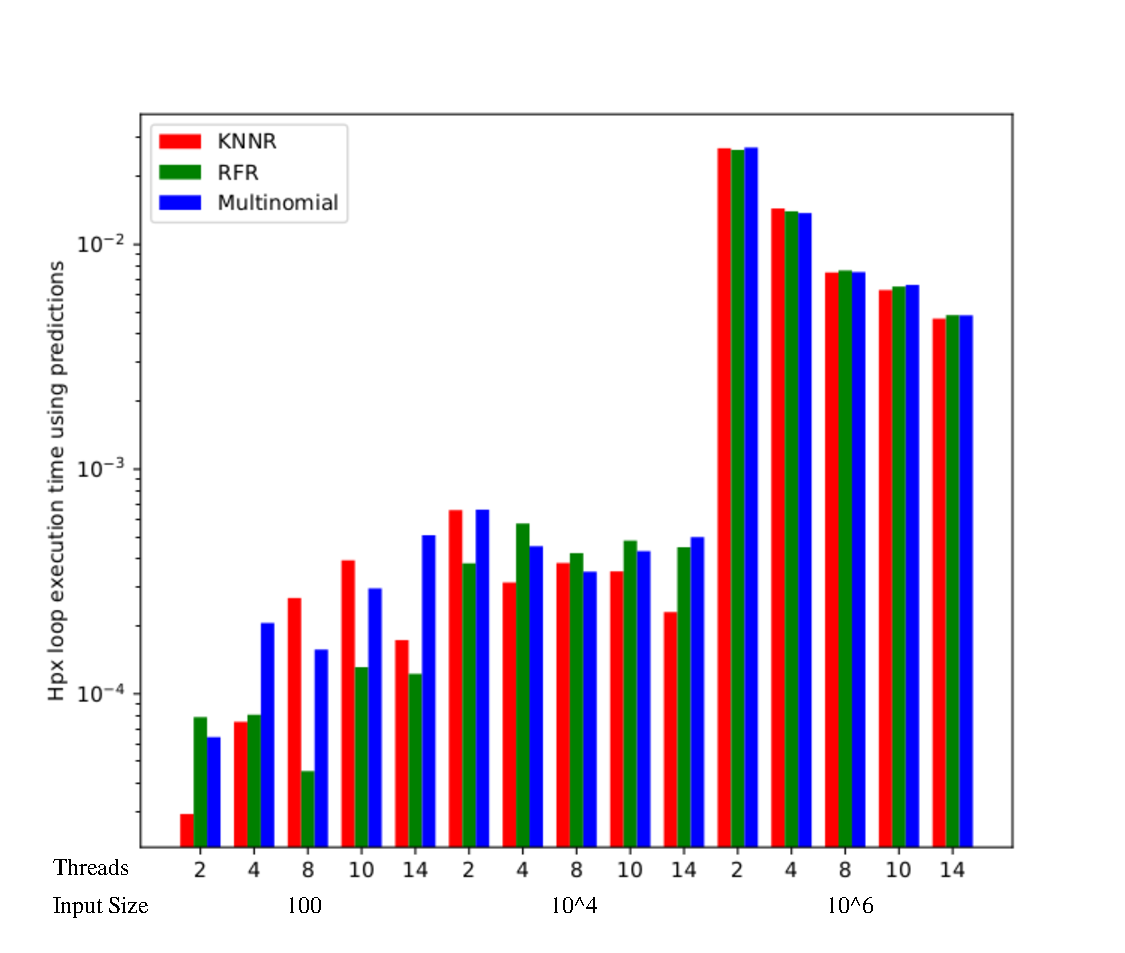
\includegraphics[width=\textwidth]{images/bars_Swap_times.pdf}
		\caption[]%
		{{HPX loops execution times}}    
	\end{subfigure}
	\caption{Chunk sizes predicted by 3 machine-learning algorithms on Swap functions (a) and the resulting Execution times measured on hpx for-loops (b)} 
\end{figure*}
Here the times are so close relative to the variance of measurement that it is hard to have conclusions based on these graphs but it seems that the Multinomial algorithm performs worse because it predicts too small chunk sizes which means we observe the overhead of splitting the job.
\newpage
\subsubsection{Matrix-Vector multiplication}

\begin{table}[h]
	\centering
	\caption{Total execution times (s) on hpx for-loops with the predictions of 3 machine learning algorithms on Matrix-Vector multiplication function using k-fold cross validation}
	\label{my-label}
	\begin{tabular}{|c|c|c|c|c|}
		\hline
		& Minimal Time&K-Nearest-Neighbors & Random Forest &Multinomial Class Corrected bias\\ \hline
		k=10  &3.774&
		3.79$\pm$0.094       & 3.92$\pm$0.062&3.84$\pm$0.1 \\ \hline
	\end{tabular}
\end{table}

\begin{figure*}[h]
	\centering
	\begin{subfigure}[b]{0.5\textwidth}
		\centering
		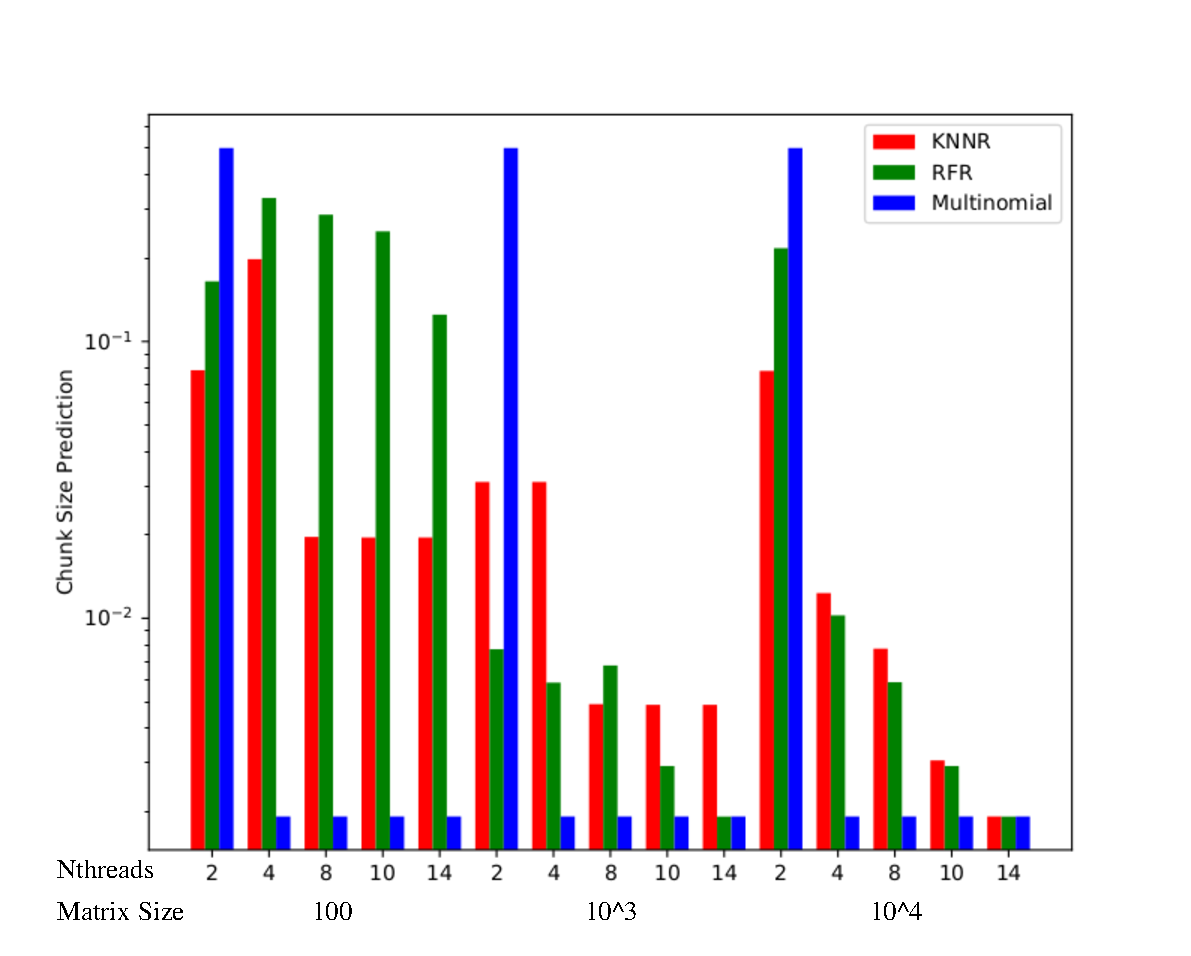
\includegraphics[width=\textwidth]{images/bars_Vector_cs.pdf}
		\caption[Network2]%
		{{Chunk sizes}}    
	\end{subfigure}
	\hfill
	\begin{subfigure}[b]{0.49\textwidth}  
		\centering 
		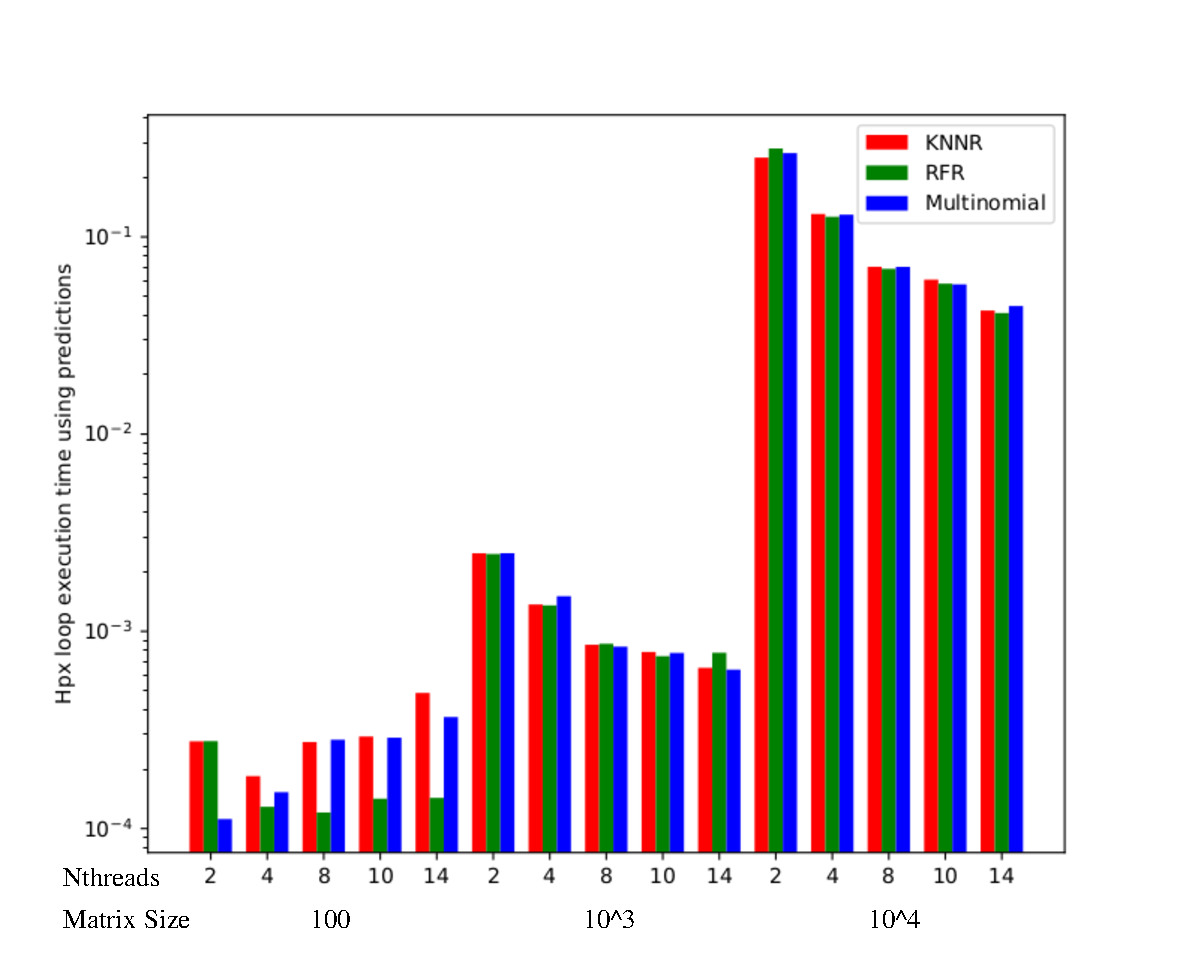
\includegraphics[width=\textwidth]{images/bars_vector_times.pdf}
		\caption[]%
		{{HPX loops execution times}}    
	\end{subfigure}
	\caption{Chunk sizes predicted by 3 machine-learning algorithms on Matrix-Vector multiplication functions (a)and the resulting Execution times measured on hpx for-loops (b)} 
\end{figure*}
here the times differences are mainly caused by variance because we see multiple instances where the predictions are all the same for 3 algorithms but we observe a difference in execution time.

\newpage
\subsubsection{Matrix-matrix multiplication}
\begin{table}[h]
	\centering
	\caption{Total execution times (s) on hpx for-loops with the predictions of 3 machine learning algorithms on Matrix-Matrix multiplication using k-fold cross validation}
	\label{my-label}
	\begin{tabular}{|c|c|c|c|c|}
		\hline
		& Minimal Time&K-Nearest-Neighbors & Random Forest &Multinomial Class Corrected bias\\ \hline
		k=10  &222.92&
		235$\pm$3       & 229$\pm$2&225$\pm$3 \\ \hline
	\end{tabular}
\end{table}

\begin{figure*}[h]
	\centering
	\begin{subfigure}[b]{0.5\textwidth}
		\centering
		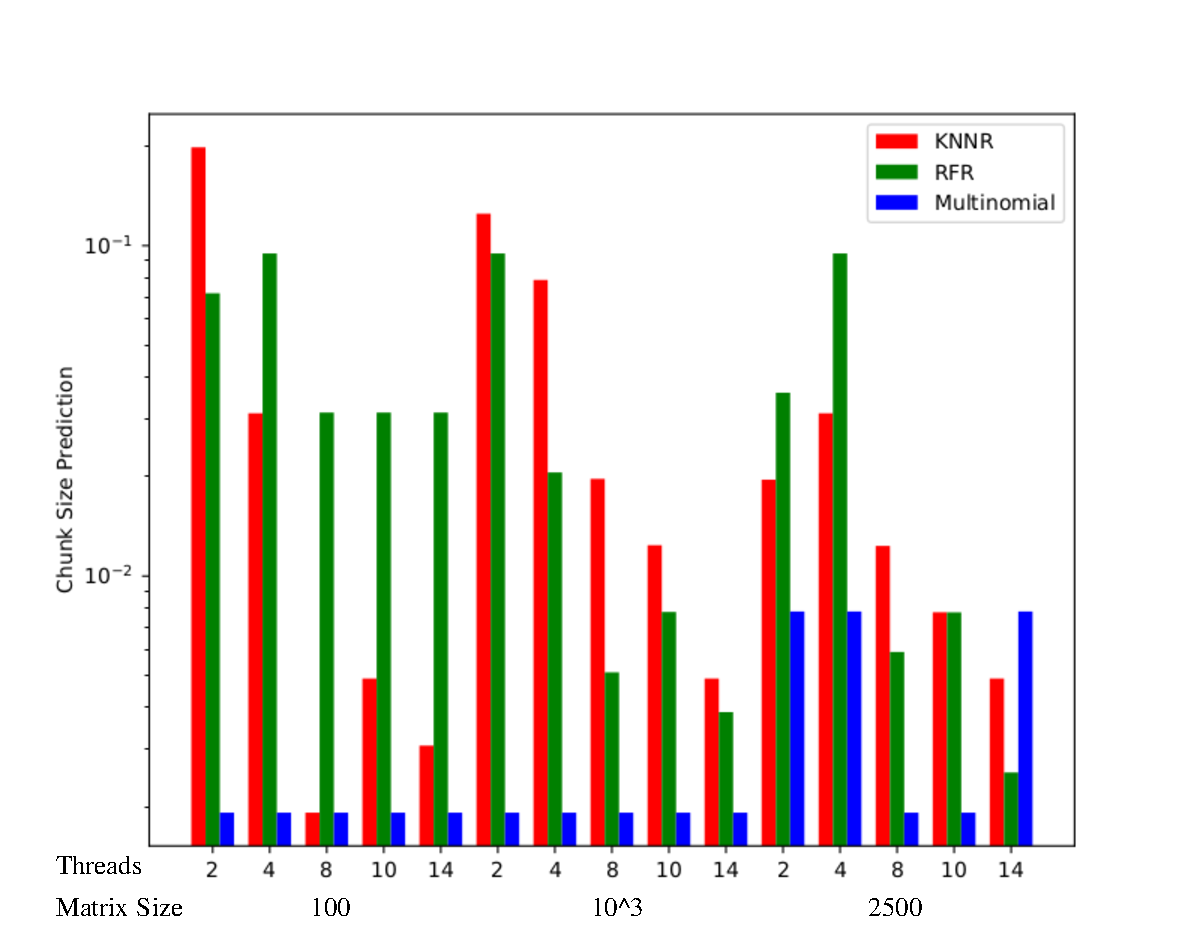
\includegraphics[width=\textwidth]{images/bars_matrix_cs.pdf}
		\caption[Network2]%
		{{Chunk sizes}}    
	\end{subfigure}
	\hfill
	\begin{subfigure}[b]{0.49\textwidth}  
		\centering 
		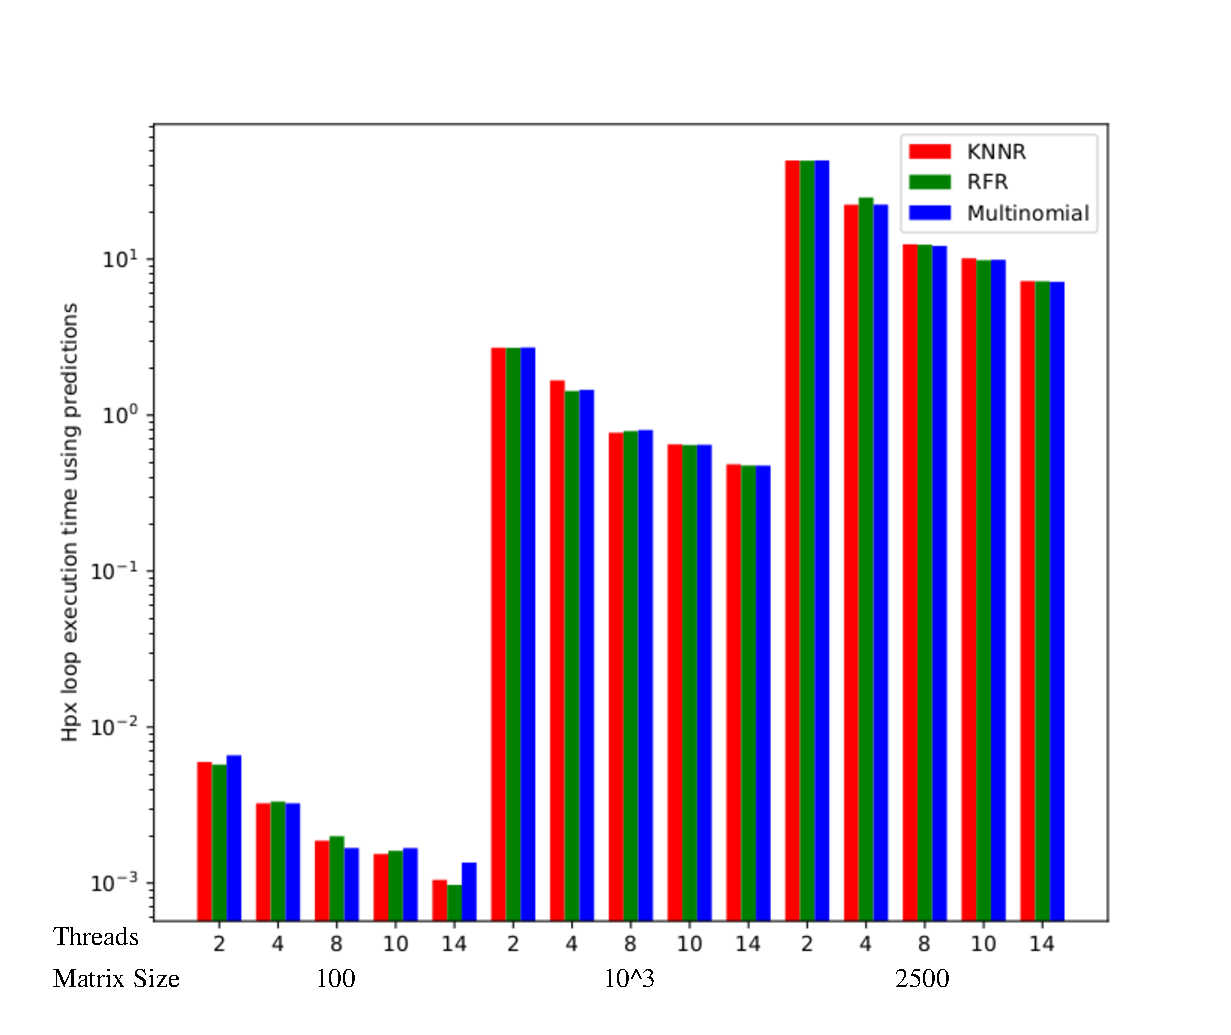
\includegraphics[width=\textwidth]{images/bars_matrix_times.pdf}
		\caption[]%
		{{HPX loops execution times}}    
	\end{subfigure}
	\caption{Chunk sizes predicted by 3 machine-learning algorithms on Matrix-Matrix multiplication functions (a) and the resulting Execution times measured on hpx for-loops (b)} 
\end{figure*}
We can see that for this function, multinomial algorithm is way better than the other two. 
\newpage
\subsubsection{Max}
\begin{table}[h]
	\centering
	\caption{Total execution times (s) on hpx for-loops with the predictions of 3 machine learning algorithms on Max using k-fold cross validation}
	\label{my-label}
	\begin{tabular}{|c|c|c|c|c|}
		\hline
		& Minimal Time&K-Nearest-Neighbors & Random Forest &Multinomial Class Corrected bias\\ \hline
		k=10  &48.432&
		79.47$\pm$1.33       & 75.52$\pm$1.53&75.7$\pm$1.72 \\ \hline
	\end{tabular}
\end{table}

\begin{figure*}[h]
	\centering
	\begin{subfigure}[b]{0.5\textwidth}
		\centering
		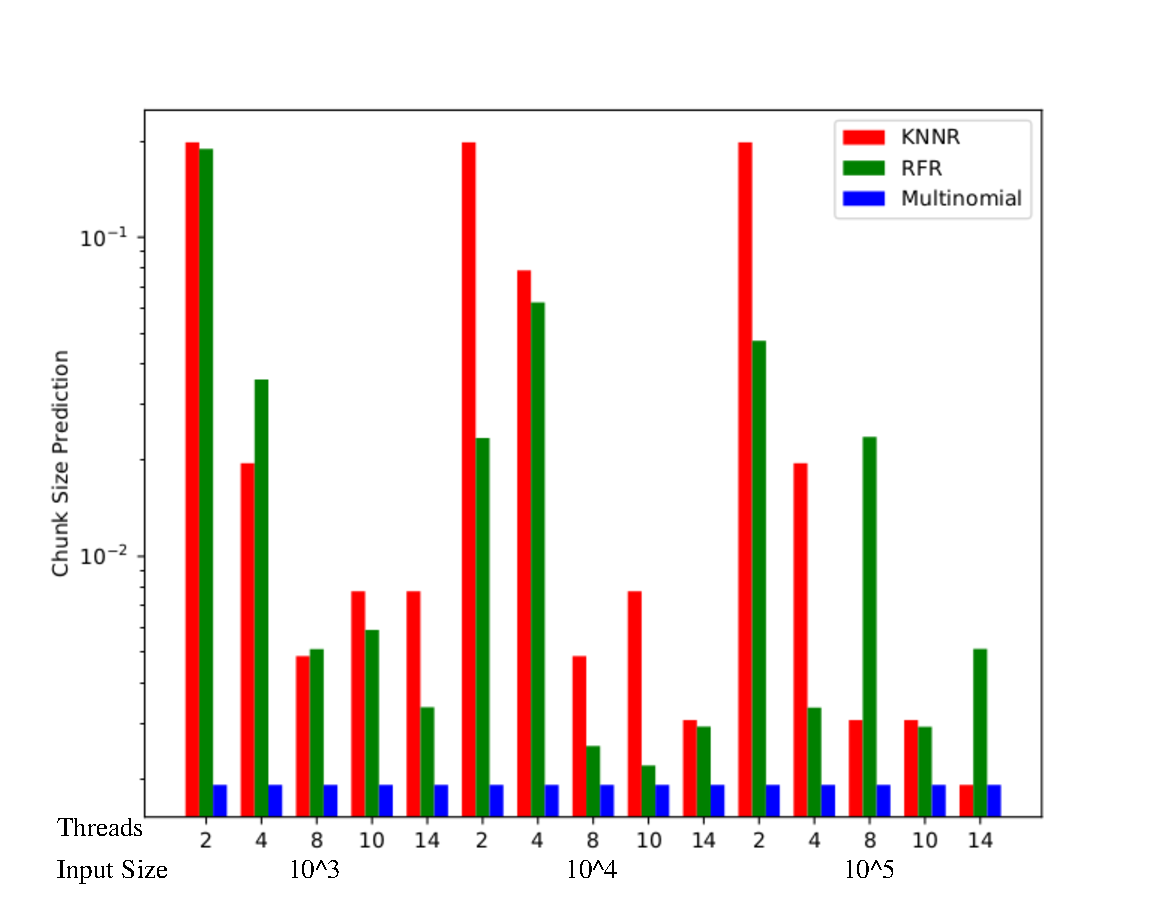
\includegraphics[width=\textwidth]{images/bars_max_cs.pdf}
		\caption[Network2]%
		{{Chunk sizes}}    
	\end{subfigure}
	\hfill
	\begin{subfigure}[b]{0.49\textwidth}  
		\centering 
		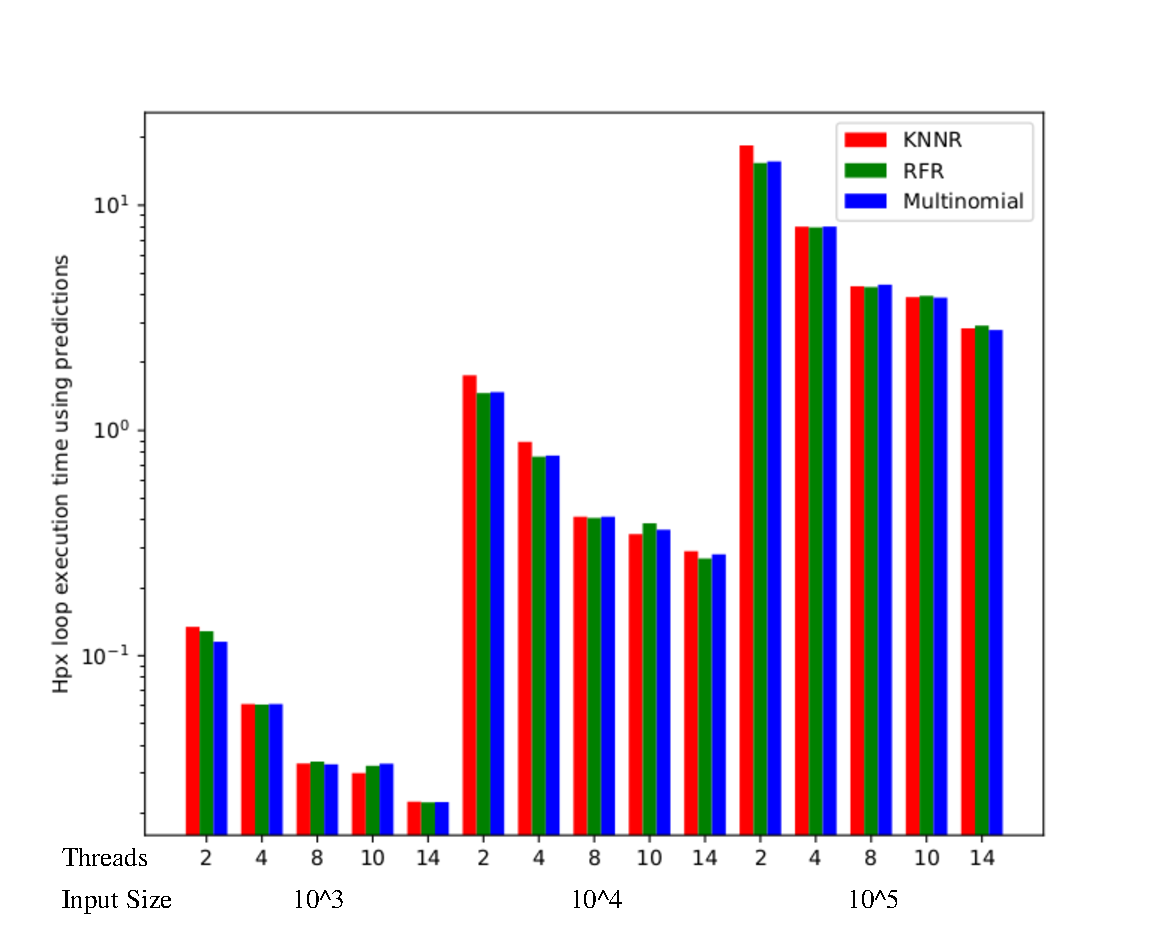
\includegraphics[width=\textwidth]{images/bars_max_times.pdf}
		\caption[]%
		{{HPX loops execution times}}    
	\end{subfigure}
	\caption{Chunk sizes predicted by 3 machine-learning algorithms on Max functions (a) and the resulting Execution times measured on hpx for-loops (b)} 
\end{figure*}
Once again we can see that multinomial only predicts small chunk sizes while other algorithms are more nuanced. This doesn't seem to affect execution time that much .
\newpage
\subsubsection{Tensor Generator}
\begin{table}[h]
	\centering
	\caption{Total execution times (s) on hpx for-loops with the predictions of 3 machine learning algorithms on Tensor generator function using k-fold cross validation}
	\label{my-label}
	\begin{tabular}{|c|c|c|c|c|}
		\hline
		& Minimal Time&K-Nearest-Neighbors & Random Forest &Multinomial Class Corrected bias\\ \hline
		k=10  &26.51&
		27.32$\pm$1.328      & 26.95$\pm$1.73&26.91$\pm$1.34 \\ \hline
	\end{tabular}
\end{table}

\begin{figure*}[h]
	\centering
	\begin{subfigure}[b]{0.5\textwidth}
		\centering
		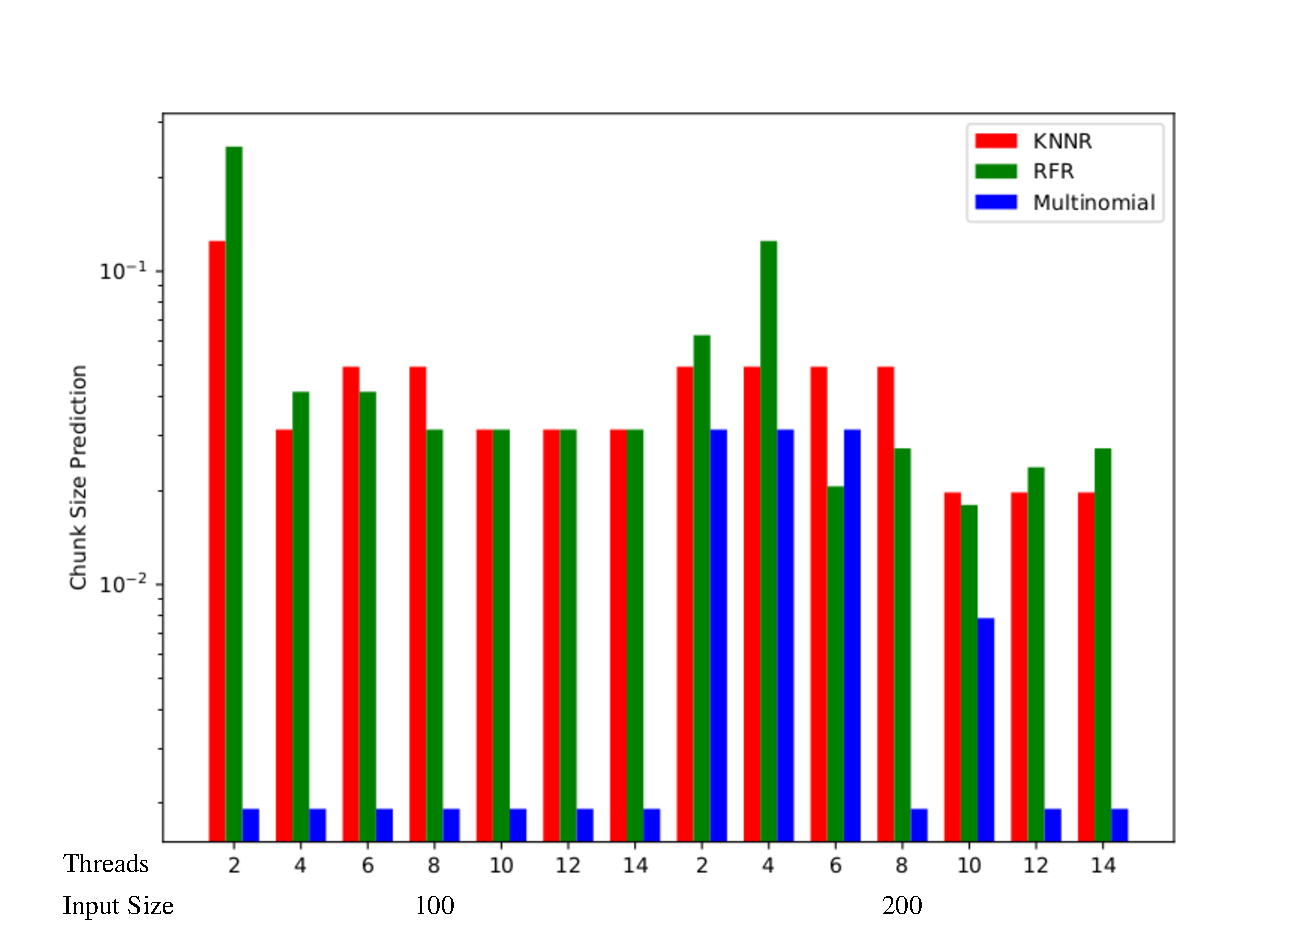
\includegraphics[width=\textwidth]{images/bars_tensor_cs.pdf}
		\caption[Network2]%
		{{Chunk sizes}}    
	\end{subfigure}
	\hfill
	\begin{subfigure}[b]{0.49\textwidth}  
		\centering 
		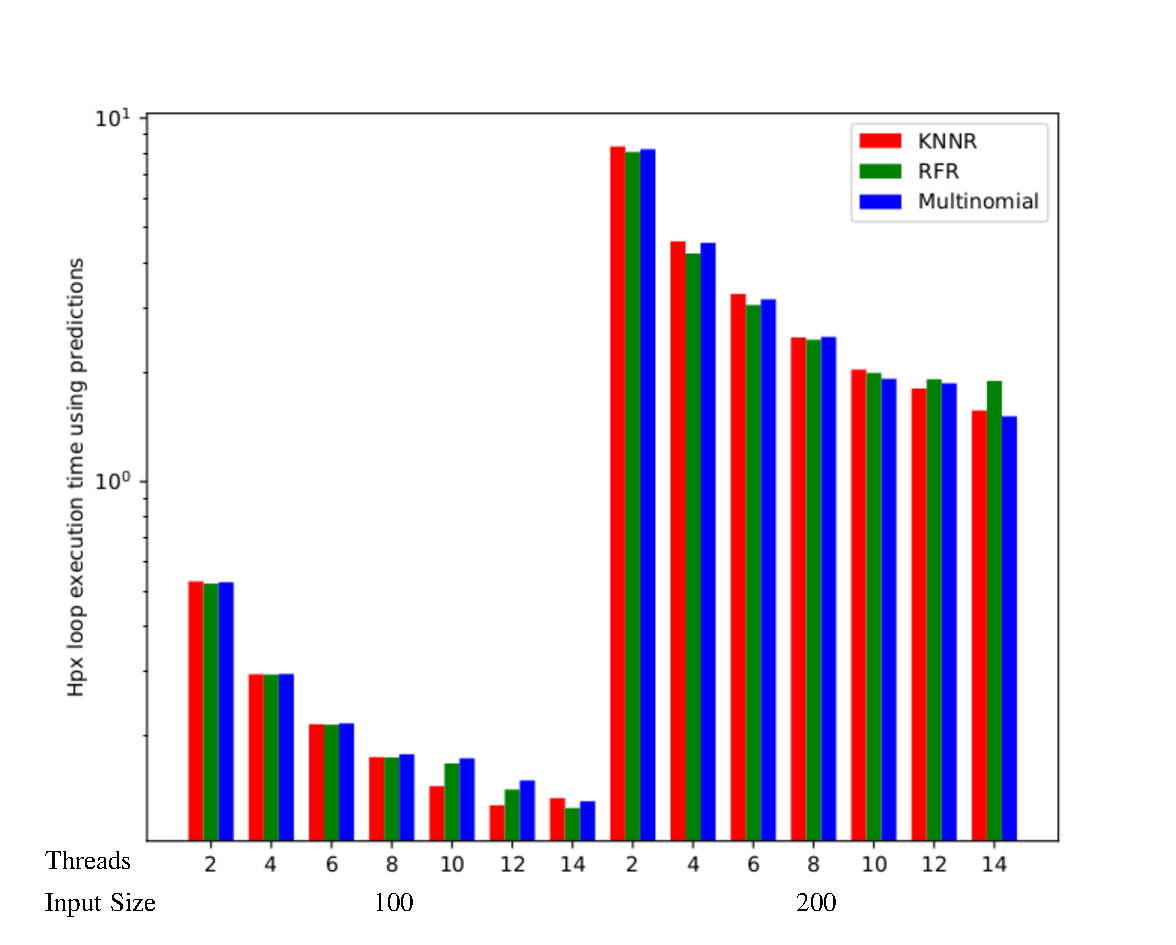
\includegraphics[width=\textwidth]{images/bars_tensor_times.pdf}
		\caption[]%
		{{HPX loops execution times}}    
	\end{subfigure}
	\caption{Chunk sizes predicted by 3 machine-learning algorithms on Tensor Generator functions (a) and the resulting Execution times measured on hpx for-loops (b)} 
\end{figure*}
Here we can see that Random Forest and Multinomial, despite differences in predictions,both have the same time.